\documentclass [a4paper, 12pt, oneside]{article}
\usepackage{fullpage}
\usepackage[utf8]{inputenc}
\usepackage{polski}
\usepackage{hyperref}
\usepackage[usenames,dvipsnames]{color}
\usepackage[pdftex]{graphicx}
\usepackage{wrapfig}
\usepackage{float}
\usepackage{amsmath}
\usepackage{amsfonts}
\linespread{1.3}
\hypersetup{
    bookmarks=true,
    unicode=false,
    pdftoolbar=true,
    pdfmenubar=true,
    pdffitwindow=false,
			        pdfstartview={FitH},
				    pdftitle={Różności o wektorach},
				        pdfauthor={Stanisław Chmiela},
					    pdfsubject={Różności o wektorach},
					        pdfcreator={Stanisław Chmiela},
						    pdfproducer={Stanisław Chmiela},
						        pdfkeywords={wektory} {matematyka},
							    pdfnewwindow=false,
							        colorlinks=true,
								    linkcolor=BrickRed,
								        citecolor=PineGreen,
									    filecolor=RawSienna,
									        urlcolor=MidnightBlue
}
\author{}
\title{Wektory}
\newcommand{\vect}[1]{\overrightarrow{#1}}
\begin{document}
\maketitle
\section{Trójkąt}

\subsection{Okrąg opisany na trójkącie}

\begin{description}
\item[Promień] $R = \frac{a}{2\sin\alpha} = \frac{abc}{4P}$
\item[Trójkąt równoboczny] $R = \frac{a\sqrt{3}}3$
\item[Trójkąt prostokątny] Trójkąt oparty na średnicy jest prostokątny.
\item[Środek] Środek okręgu opisanego znajdujemy na przecięciu symetralnych boków trójkąta.
\end{description}

\subsection{Okrąg wpisany w trójkąt}

\begin{description}
\item[Promień] $r = \frac{2P}{a+b=c}$
\item[Trójkąt równoboczny] $r = \frac{a\sqrt3}6$
\item[Trójkąt prostokątny] $r = \frac{b+a-c}2$
\item[Trójkąt równoramienny] Podstawa -- $a$, ramiona -- $b$, $r = \frac{ab-\frac12a^2}{2\sqrt{\left(b^2-\frac14a^2\right)}}$
\item[Środek] Środek okręgu wpisanego znajdujemy na przecięciu dwusiecznych kątów trójkąta.
\end{description}

\section{Czworokąt}

\subsection{Okrąg opisany na czworokącie}

\begin{description}
\item[Środek] Środek okręgu opisanego znajdujemy na przecięciu symetralnych boków.
\end{description}

\subsubsection{Warunek konieczny do opisania okręgu}
\begin{figure}[h!]
      \centering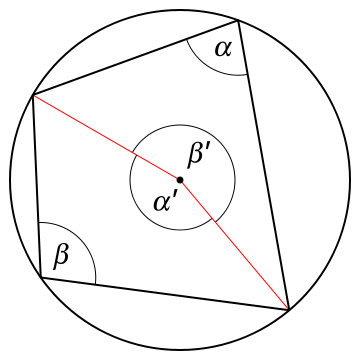
\includegraphics[width=0.38\textwidth]{Graphics/geometria1}
	  \end{figure}
\paragraph{Twierdzenie}
Okrąg można opisać na czworokącie wtedy i tylko wtedy, gdy sumy miar przeciwległych kątów czworokąta równe są $\pi$.
\paragraph{Dowód $\Rightarrow$}
Z twierdzenia o miarach kątów wpisanych i środkowych opartych na tym samym łuku miara kąta $\alpha^\prime = 2\alpha$, a kąta $\beta^\prime = 2\beta$. Jednocześnie $\alpha^\prime + \beta^\prime = 2\pi$. Zatem $\alpha + \beta = \pi$.
\paragraph{Dowód $\Leftarrow$}
Rozważmy sobie dwa przypadki, gdy czworokąta nie da się wpisać w okrąg.
\subparagraph{Wierzchołek wystaje poza okrąg}
Wtedy z twierdzenia o kątach wpisanych i środkowych opartych na tym samym łuku dostajemy, że $$\angle ADC \le \pi - 2\angle ABC$$, a zatem $$\angle ADC + \angle ABC < \pi$$.
\subparagraph{Wierzchołek jest wewnątrz okręgu}

\subsection{Okrąg wpisany w czworokąt}

Okrąg styczny do każdego z boków wielokąta.

\paragraph{Twierdzenie} Okrąg można wpisać w czworokąt wtedy i tylko wtedy, gdy sumy długości przeciwległych boków są sobie równe.
\paragraph{Dowód} Z ,,\emph{najmocniejszego twierdzenia geometrii}'' dostajemy taki rysunek, zaiste $a+b+c+d = a+b+c+d$.
\begin{figure}[h!]
      \centering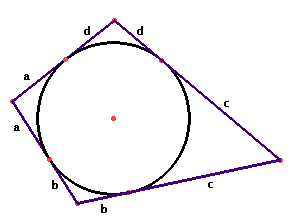
\includegraphics[width=0.5\textwidth]{Graphics/geometria2}
	  \end{figure}

\end{document}
